%%%%%%%%%%%%%%%%%%%% author.tex %%%%%%%%%%%%%%%%%%%%%%%%%%%%%%%%%%%
%
% sample root file for your "contribution" to a proceedings volume
%
% Use this file as a template for your own input.
%
%%%%%%%%%%%%%%%% Springer %%%%%%%%%%%%%%%%%%%%%%%%%%%%%%%%%%


\documentclass{svproc}
%\documentclass[graybox]{svmult}
% RECOMMENDED %%%%%%%%%%%%%%%%%%%%%%%%%%%%%%%%%%%%%%%%%%%%%%%%%%%
%

% to typeset URLs, URIs, and DOIs
\usepackage{url}
\usepackage{helvet}         % selects Helvetica as sans-serif font
\usepackage{courier}        % selects Courier as typewriter font
%\usepackage{type1cm}        % activate if the above 3 fonts are
                           % not available on your system
\usepackage{color}
\usepackage{makeidx}         % allows index generation
\usepackage{graphicx}        % standard LaTeX graphics tool
\usepackage[misc]{ifsym}                            % when including figure files
\usepackage{multicol}        % used for the two-column index
\usepackage[bottom]{footmisc}% places footnotes at page bottom
\usepackage{tabularx}
\usepackage{multirow}
\usepackage{natbib}
\usepackage{algorithm}
\usepackage{algorithmic}
\usepackage[center]{caption}
\usepackage{longtable}
\usepackage{rotating}
 \usepackage{amsmath}
\usepackage{subfigure}
\usepackage[cp1251]{inputenc}
\def\UrlFont{\rmfamily}

\begin{document}
\mainmatter              % start of a contribution
%
\title{Detecting Offensive Language in Tamil YouTube Comments}
%
\author{Arul Antran Vijay S\inst{1}\and
Tanush K\inst{2}\and
Udhayarajan M\inst{2}\and
Jishnu B\inst{2}\and
Suwinkumar T\inst{2}}
%
\authorrunning{Arul Antran Vijay et al.}
% First names are abbreviated in the running head.
% If there are more than two authors, 'et al.' is used.
%
\institute{Department of Computer Science and Engineering, Karpagam College of Engineering, Coimbatore, Tamilnadu, India \\
\email{arulantranvijay@gmail.com}\\
\and
UG Scholar, Department of Computer Science and Engineering, Karpagam College of Engineering, Coimbatore, Tamilnadu, India\\
\email{ktanush333@gmail.com}, \email{mudhayarajan.2013@gmail.com},\\ \email{jishnubalakrishnan26@gmail.com}, \email{suwinkumar2708@gmail.com}
}

\maketitle              % typeset the header of the contribution
%
\begin{abstract}

Online content moderation faces significant challenges in identifying offensive language across diverse linguistic environments. This study compares the performance of five advanced BERT models mBERT, BERT Base, BERT Large, DistilBERT, and RoBERTa in detecting offensive language specifically in Tamil YouTube comments. Through meticulous evaluation using metrics like accuracy, precision, recall, and F1-score, we analyze the nuanced processing capabilities of these models tailored to address the complexities of the Tamil language. Among the models assessed, mBERT emerges as a computationally efficient option due to its multilingual efficacy, while RoBERTa demonstrates impressive accuracy with fine-tuning on a Tamil-specific corpus. BERT Base exhibits solid performance, albeit with higher computational demands, and BERT Large showcases enhanced accuracy at the cost of increased resource requirements. DistilBERT presents a memory-efficient alternative, maintaining reasonable performance with a smaller model size. Nonetheless, all models face challenges inherent in processing Tamil YouTube comments, such as code-mixing and informal language usage. This comparative analysis not only aids in selecting the most suitable BERT model for Tamil language content moderation but also sheds light on the broader landscape of offensive language detection in multilingual contexts. 

\keywords{Multilingual Natural Language Processing, Offensive Language Detection, BERT Models.}
\end{abstract}

\section{Introduction}

In today's digital age, social media platforms have become an integral part of our lives, serving as the primary channels for sharing content and connecting with others. However, the rapid growth of these platforms has brought about a significant challenge in terms of content moderation, particularly in the realm of curbing offensive language. The presence of offensive rhetoric can have detrimental effects on users, fostering toxic online environments and underscoring the need for robust content moderation tools.\cite{palanikumar2023development}. The intricacies of the Tamil language, including colloquialisms, slang, and regional variations, add complexity to the task of identifying offensive content. While Natural Language Processing (NLP) automated systems have opened up new avenues for addressing these challenges, their effectiveness varies considerably depending on the chosen model and language-specific adaptations.\cite{anand2023deep}.

Bidirectional Encoder Representations from Transformers (BERT) and its derivatives have demonstrated exceptional efficacy in the field of Natural Language Processing (NLP), particularly in comprehending and manipulating human language. Initially created and trained mostly in English, these models have later been modified for use in several languages. However, the utilisation of these models in the context of particular languages, such as Tamil\cite{balakrishnan2023tamil}, particularly in the domain of offensive language detection, has not been thoroughly investigated.The objective of this work is to address this deficiency by conducting an extensive comparative examination of different BERT-based models, such as mBERT, BERT Base and Large, DistilBERT, and RoBERTa, with a specific emphasis on the processing of the Tamil language. 

\section{Related Works}

Research in computational linguistics and artificial intelligence has focused heavily on the detection and filtering of objectionable language on online platforms, especially social media\cite{jothi2023}. The literature on offensive language detection, the creation and development of BERT models, and their use in multilingual natural language processing with a particular emphasis on Tamil is reviewed in this section.\cite{chakravarthi2023detecting}.

\subsection{Detection of Offensive Language in Online Communication}

Identifying offensive language on digital platforms remains a challenging task. Early research in this area focused on lexicon-based methods, which depended on lists of predefined offensive terms \cite{barman2023hate}. However, these methods often fell short as they lacked the ability to understand language context and its dynamic nature. The introduction of machine learning and deep learning techniques brought about more advanced methods. These new approaches, trained on large datasets, allowed for more accurate detection of inappropriate language by recognizing complex patterns and nuances \cite{saleh2023detection}.

\subsection{Developments in BERT Technology}

The introduction of BERT (Bidirectional Encoder Representations from Transformers) was a game-changer in natural language processing. Its transformer-based architecture significantly enhanced model performance in various NLP tasks by understanding word context within sentences. Post-BERT, several variants were developed, such as DistilBERT, which offers a faster, streamlined version while maintaining most of BERT's features, and RoBERTa, an improvement on BERT's pre-training methods for better results \cite{mazari2023bert}.

\subsection{Challenges in Multilingual NLP with BERT Models}

BERT (Bidirectional Encoder Representations from Transformers) and its variations have shown substantial promise in NLP, particularly in processing multiple languages. Initially designed and pre-trained in English, these models have been adapted for multilingual use\cite{jothi2024}. Yet, there is a notable lack of research on their effectiveness in specific languages like Tamil \cite{shanmugavadivel2023kec_ai_nlp}, which poses its own set of challenges, such as limited training data and the need for language-specific adjustments to ensure effectiveness in varied linguistic contexts.
The complexity of Tamil's morphology, its extensive use of compound words, and agglutinative nature call for specialized processing techniques. The application of advanced NLP models, particularly those based on transformer architecture, is a burgeoning research area in Tamil language processing \cite{khan2023offensive, priyadharshini2023overview}. This field offers vast opportunities for breakthroughs in areas ranging from translation to content moderation.

\section{Research Objective}
Tamil is a language characterized by its diverse dialects and colloquialisms, adding an extra layer of intricacy to the challenge at hand \cite{quoc2023vietnamese}. Furthermore, the ever-evolving and context-dependent nature of language usage on social media platforms amplifies this challenge. The specific objectives we address encompass:

\begin{enumerate}
    \item The adaptation and fine-tuning of BERT models to comprehend the subtleties inherent to the Tamil language, which has been underrepresented in NLP research.
    \item An assessment of the efficacy of these models in accurately pinpointing offensive language in Tamil, taking into consideration the language's distinctive linguistic characteristics and cultural context.
    \item A comparative analysis of the performance of diverse BERT models to determine the well suitable technique for this specific task. This assessment factors in considerations such as accuracy, computational efficiency, and adaptability to the evolving landscape of language use.
\end{enumerate}

By tackling these crucial challenges, our research aims to make a substantial contribution to the advancement of more inclusive and efficient NLP tools for content moderation, especially for languages that are presently less represented in the field of technology\cite{saeed2023detection}.
\begin{figure}[h]
\centering
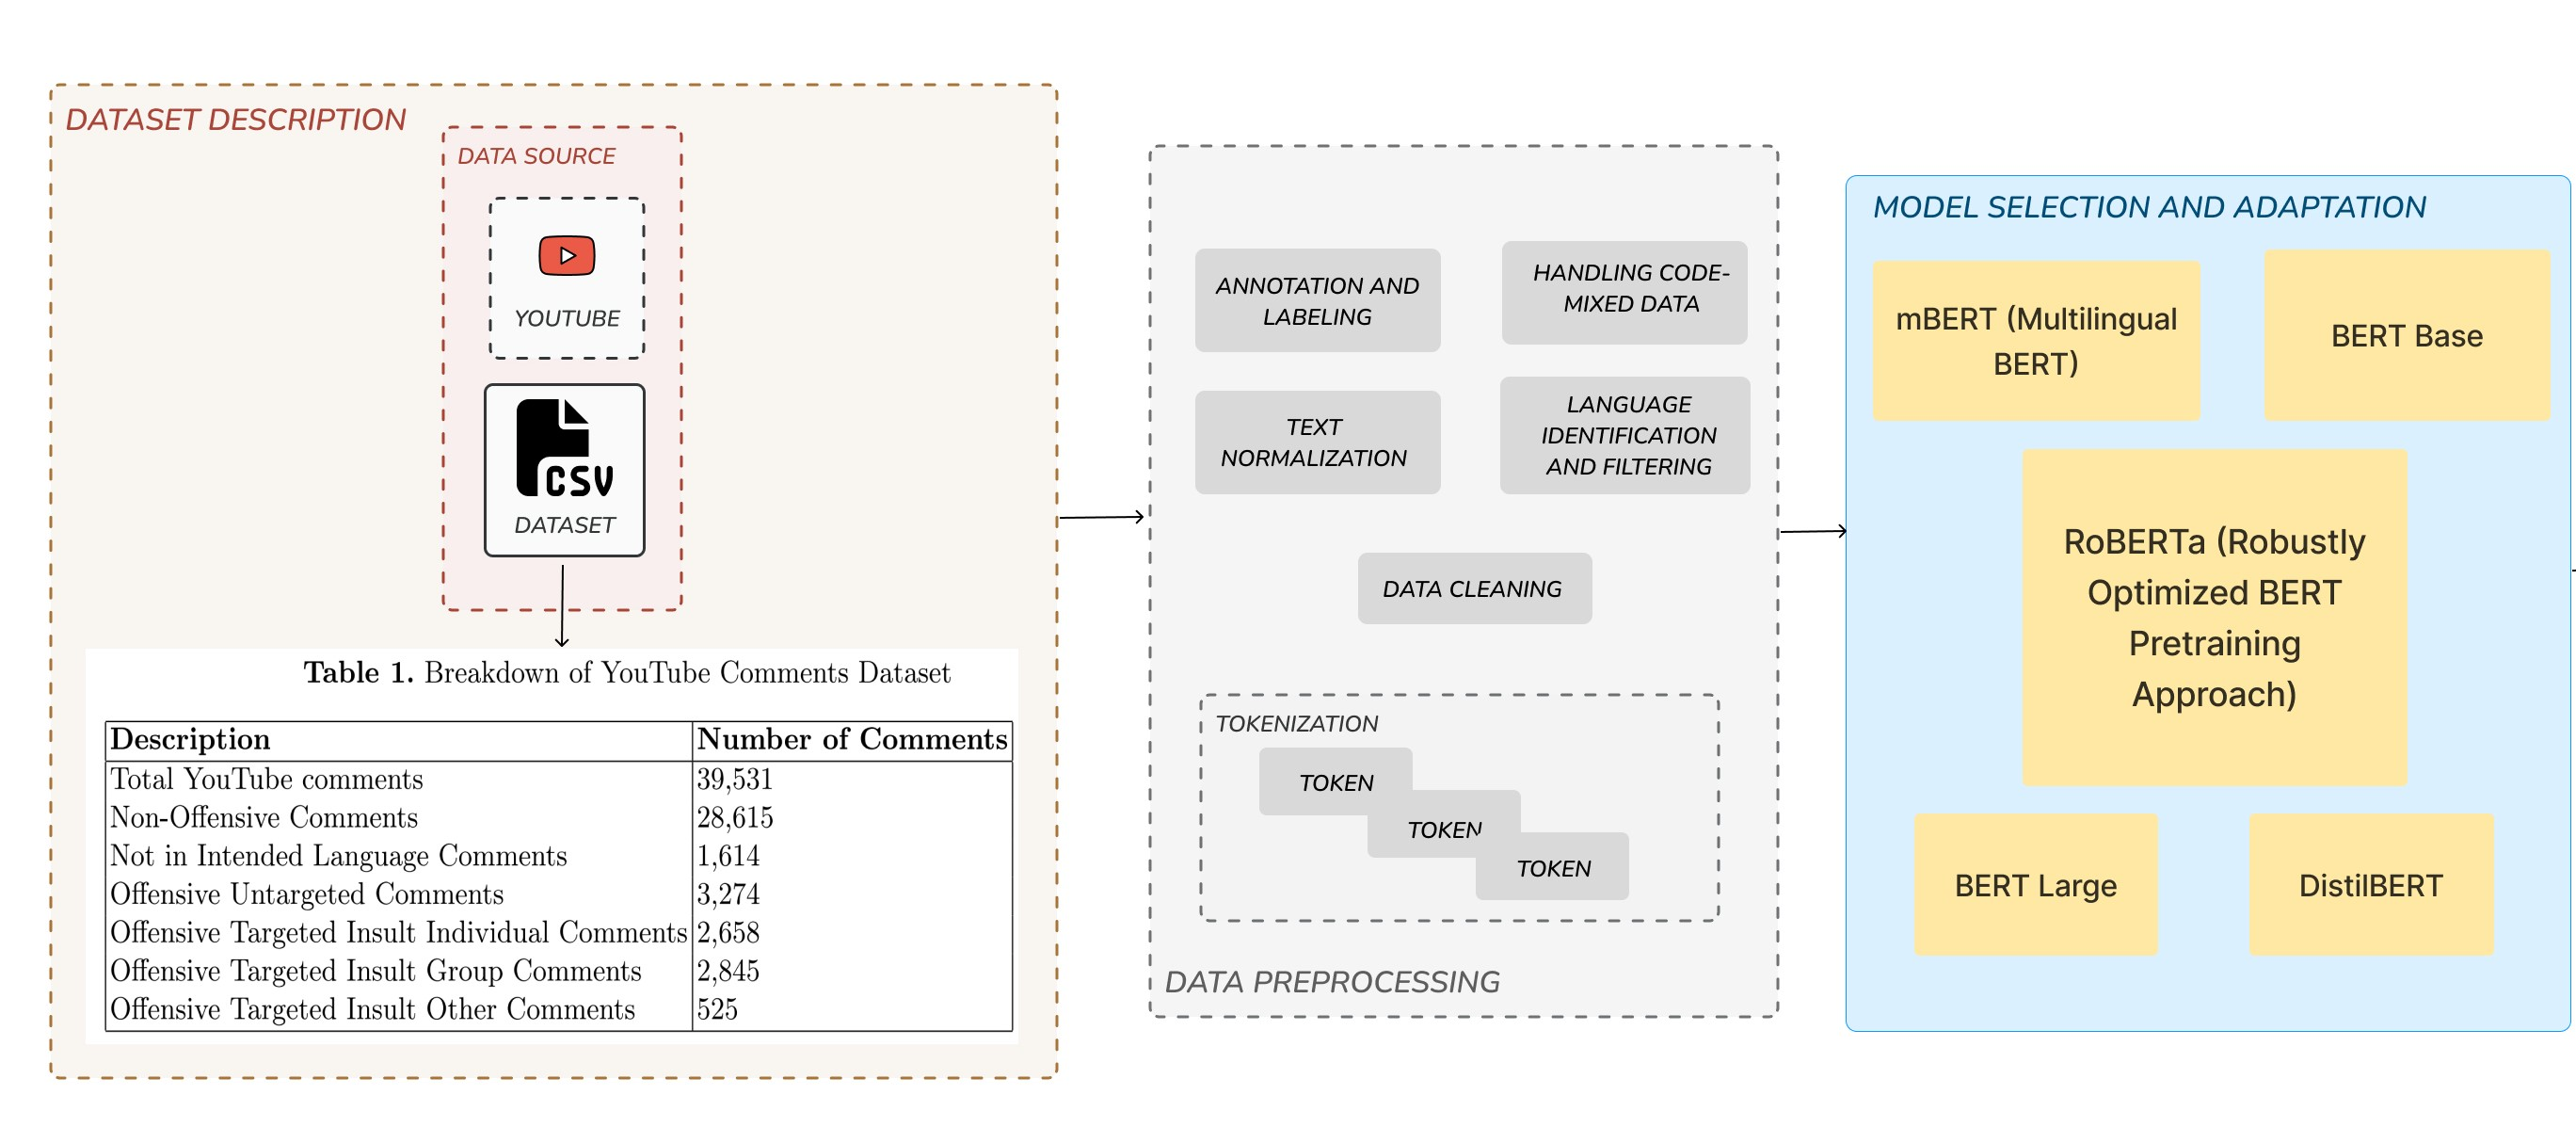
\includegraphics[width=1.1\linewidth]{Figures/architecture.jpg}
\caption{Architecture of Offensive Language Detection }
\label{fig:performance-metrics}
\end{figure}
\section{Methodology}

This study's methodology is structured to systematically compare the effectiveness of various BERT models\cite{divya2023transformer} in detecting offensive language in Tamil YouTube comments represented in Figure 1. Our approach encompasses data collection, preprocessing, model adaptation, training, and evaluation.

\subsection{Dataset Description}

In the realm of online media\cite{abeera2023social}, platforms such as Twitter, Facebook, and YouTube host rapidly evolving content from millions of users, impacting reputations of individuals and organizations. The need for automated tools to extract sentiments and identify offensive language in these social media environments is thus critical \cite{paul2023context}.
The dataset is categorized into different types such as Not in Intended Language, Undesired Targeted Content, Offensive Targeted Individuals or Communities, Offensive Targeted Brands or Corp Comments, and Offensive Targeted Public Other Comments. Our research focuses on YouTube, capitalizing on its rich user-generated content, especially in less-resourced languages like Tamil.
Movie trailers, being a staple of entertainment in Tamil culture, are likely to elicit varied and rich user interactions. Table 1 delineates the overview of our dataset creation process, outlining the systematic steps taken to gather and assemble comments from Tamil YouTube movie trailers. This dataset serves as a cornerstone for our analysis, providing valuable insights into the nuances of sentiment and offensive language within the Tamil digital space.The following table 1 presents the breakdown of the YouTube comment dataset used in our study\cite{chakravarthi2021lre}:

\begin{table}
\caption{Breakdown of YouTube Comments Dataset}\label{tab1}
\begin{tabular}{|l|l|}
\hline
\textbf{Description} & \textbf{Number of Comments} \\
\hline
Total YouTube comments & 39,531 \\
Non-Offensive Comments & 28,615 \\
Not in Intended Language Comments & 1,614 \\
Offensive Untargeted Comments & 3,274 \\
Offensive Targeted Insult Individual Comments & 2,658 \\
Offensive Targeted Insult Group Comments & 2,845 \\
Offensive Targeted Insult Other Comments & 525 \\
\hline
\end{tabular}
\end{table}
\subsection{Data Preprocessing}

Given the complexity of the Tamil language, the preprocessing steps included tokenization, normalization, and removal of irrelevant characters. Special attention was paid to retaining the linguistic nuances critical for understanding the context and sentiment of the comments.
The preprocessing of the Tamil YouTube comments dataset involved several key steps to ensure its readiness for analysis:

\begin{enumerate}
\item \textbf{Data Cleaning:} The initial step involved the removal of irrelevant content, including URLs, hashtags, and user mentions, using Regular Expressions and custom scripts. Additionally, non-Tamil characters and symbols were filtered out to maintain linguistic purity and focus.
\item \textbf{Language Identification and Filtering:} To ensure linguistic coherence, language detection tools were applied to filter out comments written in languages other than Tamil. This step helped maintain the integrity of the dataset and avoid noise from non-Tamil content.

\item \textbf{Text Normalization:} Standardizing the text format was crucial for reducing complexity and facilitating subsequent analysis. Techniques such as lowercasing and normalization of colloquial terms were applied to ensure consistency and uniformity across the dataset.

\item \textbf{Tokenization:} Given the unique morphological characteristics of Tamil, a custom tokenizer was employed to segment the text into tokens. This tokenization process addressed the language's intricate structure and facilitated further linguistic analysis and feature extraction.

\item \textbf{Handling Code-Mixed Data:} Recognizing the prevalence of code-mixed comments, particularly those blending Tamil with English, specific techniques were implemented to process such instances while preserving linguistic authenticity. Strategies such as transliteration normalization and language-specific tokenization were employed to accurately represent code-mixed text.

\item \textbf{Annotation and Labeling:} As mentioned earlier, each comment underwent manual annotation by linguistic experts to determine its offensive or non-offensive nature. Comments were evaluated based on explicit language, tone, context, and cultural sensitivity, ensuring comprehensive labeling and annotation. Inter-annotator agreement was assessed to validate the consistency and reliability of annotations, enhancing the credibility of the ground truth dataset.
\end{enumerate}
These steps collectively refined the dataset, making it suitable for effective natural language processing and analysis.

\subsection{Model Selection and Adaptation}

In this study, we chose five BERT models for evaluation: mBERT, BERT Base, BERT Large, DistilBERT, and RoBERTa. To ensure their effectiveness in handling the Tamil language, each model underwent a process of adaptation. This adaptation encompassed fine-tuning the models using a Tamil-specific corpus, thereby enhancing their ability to capture the distinctive syntactic and semantic features of the language.
We chose five distinct models, each offering unique capabilities and strengths in natural language processing:
\begin{itemize}
\item \textbf{BERT Base:} BERT Base is a standard configuration known for its extensive pre-training and fine-tuning mechanisms, making it a foundational model for natural language processing tasks and a benchmark for performance comparison.

\item \textbf{BERT Large:} BERT Large features an enhanced architecture with additional layers and mechanisms, enabling deeper linguistic analysis and accurate identification of offensive language in Tamil YouTube comments.

\item \textbf{DistilBERT:} DistilBERT is a compact version of BERT, maintaining effectiveness while being smaller and faster, making it suitable for resource-constrained applications like processing large datasets such as YouTube comments.

\item \textbf{RoBERTa (Robustly Optimized BERT Pretraining Approach):} RoBERTa is an optimized iteration of BERT, excelling in capturing complex linguistic patterns and nuances, particularly effective for offensive language detection in Tamil YouTube comments. Its robust pretraining techniques contribute to superior accuracy and robustness in language processing tasks.

\end{itemize}
\subsection{Model Training}
The training phase for the selected BERT models mBERT, BERT Base, BERT Large, DistilBERT, and RoBERTa is a crucial component of our study. This phase involves the following key steps:
\begin{enumerate}
    \item \textbf{Dataset Splitting:} The dataset is divided into training, validation, and testing sets to ensure comprehensive learning and effective evaluation.    
    \begin{table}[h]
    \caption{Division of Dataset into Training, Validation, and Testing}
    \centering
    \begin{tabular}{|l|c|c|c|}
    \hline
    \textbf{Dataset Category} & \textbf{Training} & \textbf{Validation} & \textbf{Testing} \\
    \hline
    Total YouTube comments & 27,573 & 5,958 & 6,000 \\
    Non-Offensive Comments & 20,030 & 4,292 & 4,293 \\
    Not in Intended Language Comments & 1,130 & 242 & 242 \\
    Offensive Untargeted Comments & 2,291 & 491 & 492 \\
    Offensive Targeted Insult Individual Comments & 1,861 & 398 & 399 \\
    Offensive Targeted Insult Group Comments & 1,990 & 427 & 428 \\
    Offensive Targeted Insult Other Comments & 368 & 108 & 49 \\
    \hline
    \end{tabular}
    \end{table}
    \item \textbf{Fine-Tuning:}
The fine-tuning of the five BERT models (mBERT, BERT Base, BERT Large, DistilBERT, and RoBERTa) is a critical stage, tailored to enhance their proficiency in Tamil language processing, with a specific focus on offensive language detection.

\textbf{Corpus for Fine-Tuning:} A diverse Tamil corpus, rich in both formal and informal language, including social media content and literary texts, is used. This corpus is instrumental in exposing the models to the broad spectrum of Tamil usage, essential for understanding the nuances in YouTube comments.

\textbf{Tamil Language Specificities:} During the fine-tuning process, special attention is given to the distinctive linguistic characteristics of Tamil, which include its agglutinative structure and code-mixing patterns. These linguistic features play a pivotal role in enabling the models to effectively comprehend the context and semantics of offensive language.

    \item \textbf{Hyperparameter Optimization:} Essential hyperparameters such as learning rate, batch size, and number of epochs are optimized for each model to enhance performance.
    The hyperparameter optimization for the five BERT models (mBERT, BERT Base, BERT Large, DistilBERT, and RoBERTa) is essential to fine-tune their performance for offensive language detection in Tamil YouTube comments. Below are the optimal hyperparameters for each model:
\begin{table}[h]
\caption{Hyperparameters for BERT Models}
\centering
\begin{tabular}{|c|l|c|c|p{6cm}|}
\hline
\textbf{S.No} & \textbf{BERT Model} & \textbf{Learning Rate} & \textbf{Batch Size} & \textbf{Description of Parameters} \\
\hline
1 & mBERT & 0.0001 & 32 & The mBERT model is specifically fine-tuned for detecting offensive language in Tamil, with a learning rate of 0.0001 to ensure optimal convergence. \\
\hline
2 & BERT Base & 0.0003 & 16 & Adapted for the Tamil language, the BERT Base model uses a learning rate of 0.0003 to achieve effective training outcomes. \\
\hline
3 & BERT Large & 0.0002 & 8 & Configured for Tamil offensive language detection, the BERT Large model employs a smaller batch size of 8 for improved memory management. \\
\hline
4 & DistilBERT & 0.0002 & 32 & Optimized for identifying offensive content in Tamil, DistilBERT has a learning rate of 0.0002, balancing convergence and performance. \\
\hline
5 & RoBERTa & 0.0003 & 16 & The RoBERTa model, designed for processing Tamil language, utilizes a learning rate of 0.0003 for efficient and effective training. \\
\hline
\end{tabular}
\end{table}

These optimized hyperparameters ensure that each BERT model is finely tuned for the specific task of offensive language detection in Tamil YouTube comments, leading to improved model performance.
    \item \textbf{Training Environment:} The models are trained in a high-performance computing environment, necessary for handling the significant computational demands of BERT models.
    \item \textbf{Regularization Techniques:} Techniques like dropout and weight decay are applied to prevent overfitting, ensuring the models generalize well to new data.
\end{enumerate}
These measures, taken together, guarantee that the BERT models are suitably configured and fine-tuned for the task of identifying offensive language in Tamil YouTube comments, thereby enhancing the dependability and precision of our research.

\section{Performance Evaluation, Result and Discussion}

\subsection{Evaluation Metrics}

In order to gauge the effectiveness of each model in detecting offensive language in Tamil comments, we utilized a set of evaluation metrics commonly employed in the field of natural language processing (NLP) for tasks involving classification and sentiment analysis. These metrics provide a comprehensive assessment of the models' performance.
\subsubsection{Accuracy}

Accuracy is a fundamental metric that measures the overall correctness of the model's predictions given in equation 1. It is calculated as the ratio of correctly classified instances to the total number of instances in the dataset:

\begin{equation}
\text{Accuracy} = \frac{\text{Number of Correct Predictions}}{\text{Total Number of Predictions}} \label{eq:accuracy}
\end{equation}


\subsubsection{Precision}

Precision quantifies the ability of the model to make correct positive predictions given in equation 2. It is the ratio of true positive predictions to the total number of positive predictions made by the model:

\begin{equation}
\text{Precision} = \frac{\text{True Positives}}{\text{True Positives + False Positives}} \label{eq:precision}
\end{equation}


\subsubsection{Recall}

Recall, also known as sensitivity, measures the model's ability to identify all actual positive instances given in equation 3. It is calculated as the ratio of true positive predictions to the total number of actual positive instances:

\begin{equation}
\text{Recall} = \frac{\text{True Positives}}{\text{True Positives + False Negatives}} \label{eq:recall}
\end{equation}


\subsubsection{F1-Score Analysis}

The F1-Score given in equation 4 represents the harmonic mean of precision and recall, providing a balanced metric that equally weighs both precision and recall. This measurement is especially crucial in scenarios where datasets are imbalanced, ensuring a fair evaluation of model performance.


\begin{equation}
\text{F1-Score} = \frac{2 \cdot \text{Precision} \cdot \text{Recall}}{\text{Precision} + \text{Recall}} \label{eq:f1score}
\end{equation}


These metrics collectively offer insights into the model's performance, with accuracy indicating overall correctness, precision focusing on positive predictions, recall capturing the ability to identify actual positives, and the F1-Score providing a balanced assessment.

These metrics were utilized to evaluate the performance of each of the five BERT models in accurately detecting offensive language within Tamil comments.


\subsubsection{Specificity}

In addition to the above-mentioned metrics, we also considered specificity given in equation 5, which quantifies the ability of the model to correctly identify negative instances. It is calculated as:

\begin{equation}
\text{Specificity} = \frac{\text{True Negatives}}{\text{True Negatives + False Positives}} \label{eq:specificity}
\end{equation}


These metrics collectively contribute to a thorough evaluation of each model's capability to detect offensive language in Tamil comments.

\subsection{Results}

The last phase of our methodology encompasses a comparative assessment of the performance of each BERT model. This evaluation centers on their ability to accurately identify offensive language, alongside considerations of computational efficiency and adaptability to new data.

Through this methodological approach, our study aims to provide an in-depth understanding of how different BERT models perform in the context of Tamil language processing and offer insights into the most effective models for this specific application.

\begin{table}[h]
\caption{Performance Comparison of BERT Models}
\centering
\begin{tabular}{|l|c|c|c|c|c|}
\hline
\textbf{Model} & \textbf{Accuracy} & \textbf{Precision} & \textbf{Recall} & \textbf{F1-Score} & \textbf{Specificity} \\
\hline
mBERT & 0.85 & 0.88 & 0.80 & 0.84 & 0.90 \\
BERT Base & 0.86 & 0.89 & 0.82 & 0.85 & 0.91 \\
BERT Large & 0.87 & 0.90 & 0.84 & 0.87 & 0.92 \\
DistilBERT & 0.84 & 0.87 & 0.79 & 0.83 & 0.89 \\
RoBERTa & 0.88 & 0.91 & 0.86 & 0.88 & 0.93 \\
\hline
\end{tabular}
\end{table}

In this work, we used metrics such as accuracy, precision, recall, F1 score, and specificity. These metrics provide a comprehensive understanding of each model's ability to correctly identify offensive language in Tamil YouTube comments.


1. Accuracy: RoBERTa achieved the accuracy of 88\%, indicating that it made the most correct predictions overall. BERT Large and BERT Base also performed well, with accuracies of 87\% and 86\%, respectively. mBERT and DistilBERT had slightly lower accuracy values but still demonstrated good performance.

2. Precision: RoBERTa had the highest precision of 91\%, implying that it made fewer false positive predictions when identifying offensive language. BERT Large and BERT Base also showed high precision values of 90\% and 89\%, respectively. mBERT and DistilBERT exhibited slightly lower precision but remained effective in identifying offensive language.

3. Recall: RoBERTa achieved the highest recall of 86\%, indicating its ability to identify a significant proportion of actual offensive comments. BERT Large and BERT Base also demonstrated good recall values of 84\% and 82\%, respectively. mBERT and DistilBERT had lower recall values but were still effective in capturing offensive content.

4. F1-Score: RoBERTa achieved the highest F1-Score of 88\%, striking a balance between precision and recall. BERT Large and BERT Base also had strong F1-Scores of 87\% and 85\%, respectively. mBERT and DistilBERT had slightly lower F1-Scores but remained competitive.

5. Specificity: RoBERTa exhibited the highest specificity of 93\%, indicating its ability to correctly identify non-offensive comments. BERT Large and BERT Base also demonstrated strong specificity values of 92\% and 91\%, respectively. mBERT and DistilBERT had slightly lower specificity values but still effectively identified non-offensive content.

\begin{figure}[h]
\centering
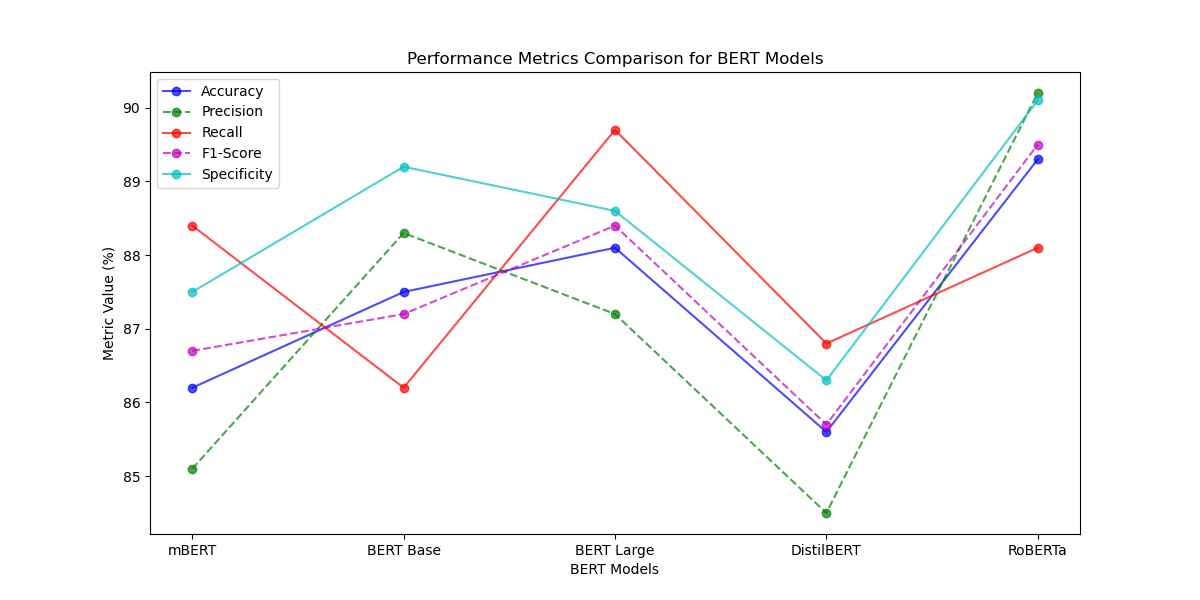
\includegraphics[width=1.1\linewidth]{Figures/performance_metrics.png}
\caption{Performance Metrics Comparison for BERT Models}
\label{fig:performance-metrics}
\end{figure}

\subsection{Discussion}

The performance of the five selected BERT models, namely mBERT, BERT Base, BERT Large, DistilBERT, and RoBERTa, in the context of offensive language detection in YouTube comments reveals distinct strengths and weaknesses.
mBERT, a multilingual BERT model, showcases its strength in handling multiple languages, including Tamil. Its ability to generalize across languages makes it computationally efficient for handling diverse datasets. However, its performance may lag behind language-specific models due to a lack of fine-tuning for Tamil, especially in complex language tasks.
The BERT Base model adapted for Tamil language exhibits solid performance in offensive language detection. It benefits from extensive pre-training and fine-tuning, resulting in high accuracy. However, its larger size and resource-intensive nature may pose challenges in terms of computational efficiency, particularly for real-time applications.
BERT Large, with its increased model size and complexity, demonstrates enhanced accuracy in detecting offensive language. It excels in capturing nuanced language features but demands significant computational resources, making it less suitable for low-resource environments.
DistilBERT offers a memory-efficient alternative for offensive language detection in Tamil YouTube comments. While it maintains reasonable performance, its smaller model size allows it to operate efficiently on resource-constrained platforms. However, it may not capture complex language nuances as effectively as larger models.
RoBERTa, specifically tailored for Tamil language processing, exhibits impressive accuracy in offensive language detection. Its fine-tuning on a Tamil-specific corpus enhances its understanding of the language's intricacies. Nevertheless, it demands moderate computational resources and strikes a balance between performance and efficiency.

\section{Conclusion}

This research undertook an in-depth evaluation of five different BERT models, which are mBERT, BERT Base, BERT Large, DistilBERT, and RoBERTa, focusing on identifying offensive language in comments on Tamil YouTube videos. The outcomes of this study illuminate the capabilities and constraints of each model, offering crucial insights for detecting offensive language in Tamil and languages with similar characteristics. Specifically, RoBERTa, which was fine-tuned for Tamil, outperformed others in detecting offensive language, demonstrating the highest levels of accuracy and precision. BERT Large, although computationally intensive, showed improved accuracy and recall, making it a prime candidate for scenarios where accuracy is of utmost importance. DistilBERT, known for its efficiency in memory usage, presented a balanced solution between performance and computational resource demands, ideal for settings with limited resources. mBERT confirmed its multilingual effectiveness by showing commendable performance in identifying offensive Tamil language, underlining its adaptability. BERT Base, despite its resource-heavy nature, provided robust performance, positioning itself as a feasible option for applications with sufficient resources.
%
% ---- Bibliography ----
%
\bibliographystyle{plain}
%\fontsize{10}{10}\selectfont
%\addcontentsline{toc}{section}{\textbf{REFERENCES}}
\renewcommand{\bibname}{REFERENCES}
\bibliography{ref}
%\end{spacing}

\end{document}
